% Rationalisation: committing to a response before the mix is revealed.
% Shared preamble for the write-on class slides.
%
% Every deck is designed to be projected and annotated live on a tablet:
% whatever takes time to draw is pre-drawn, and whatever the class produces is
% left blank. Compile a deck with `pdflatex main.tex` from its own directory,
% or run `make` in decks/ to build them all.
\documentclass[10pt]{article}

\usepackage[papersize={25.6cm,14.4cm}, margin=1.1cm, bottom=1.5cm,
            footskip=0.75cm]{geometry}
\usepackage[T1]{fontenc}
\usepackage[default]{sourcesanspro}
\usepackage{newtxsf}
\usepackage{tikz}
\usepackage{amsmath}
\usepackage{parskip}
\usepackage{fancyhdr}
\usetikzlibrary{arrows.meta, positioning, calc}

\setlength{\parindent}{0pt}

% Catppuccin Latte, the palette the course site uses in its light theme, so a
% deck on the projector looks like the pages the students read.
\definecolor{inkbg}{HTML}{EFF1F5}      % base
\definecolor{inksurface}{HTML}{E6E9EF} % mantle
\definecolor{inkfaint}{HTML}{CCD0DA}   % surface2, for rules and empty boxes
\definecolor{inktext}{HTML}{4C4F69}    % text
\definecolor{inkgrey}{HTML}{8C8FA1}    % overlay1, for anything secondary
\definecolor{inkblue}{HTML}{7287FD}    % lavender, the primary accent
\definecolor{inkteal}{HTML}{179299}    % teal
\definecolor{inkred}{HTML}{FE640B}     % peach, for whatever wants attention
\definecolor{inkmauve}{HTML}{8839EF}   % mauve

\pagecolor{inkbg}
\color{inktext}

% A box to write a number into. White against the tinted page, so it reads as
% somewhere to write rather than as part of the printed material.
\newcommand{\blank}[1][1.6]{%
  \tikz[baseline=(current bounding box.base)]{%
    \draw[inkfaint, line width=0.7pt, rounded corners=2pt, fill=white]
      (0,-0.18) rectangle (#1,0.62);}}

% A ruled area to work in. Faint dots keep handwriting level on a tablet.
\newcommand{\workspace}[2]{%
  \begin{tikzpicture}
    \draw[inkfaint, line width=0.7pt, rounded corners=3pt, fill=white]
      (0,0) rectangle (#1,#2);
    \foreach \gx in {0.5,1.0,...,#1}{%
      \foreach \gy in {0.5,1.0,...,#2}{%
        \fill[inkfaint] (\gx,\gy) circle (0.5pt);}}
  \end{tikzpicture}}

% A panel for material that is printed rather than written on.
\newcommand{\panel}[2]{%
  \begin{tikzpicture}
    \draw[inkfaint, line width=0.7pt, rounded corners=3pt, fill=inksurface]
      (0,0) rectangle (#1,#2);
  \end{tikzpicture}}

% An empty payoff grid. #1 is the list of action names, #2 is drawn afterwards
% so a page can add its own marks.
\newcommand{\payoffgrid}[2]{%
  \begin{tikzpicture}[scale=1.0, every node/.style={transform shape}]
    \foreach \name [count=\j from 0] in {#1}{%
      \node[font=\bfseries, text=inkblue] at (\j*2.7+1.35,0.55) {\name};
      \node[font=\bfseries, text=inkblue] at (-1.15,-\j*2-1) {\name};
      \foreach \k [count=\i from 0] in {#1}{%
        \draw[inkfaint, line width=0.7pt, fill=white]
          (\j*2.7,-\i*2) rectangle (\j*2.7+2.7,-\i*2-2);}}
    #2
  \end{tikzpicture}}

% The five actions on a pentagon. Each action beats the one next to it and the
% one across from it, so the two winning cycles are drawn as separate panels:
% ten labelled arrows on one diagram is a tangle nobody can read from the back
% of the room.
\newcommand{\rpslscycle}[3]{%
  \begin{tikzpicture}[scale=1.0, every node/.style={transform shape},
      >={Stealth[length=2.6mm]},
      action/.style={circle, draw=inkfaint, line width=1pt, fill=white,
                     text=inktext, minimum size=1.7cm, inner sep=1pt,
                     font=\small\bfseries},
      beats/.style={->, line width=1.2pt, shorten >=3pt, shorten <=3pt,
                    draw=#1},
      word/.style={font=\scriptsize, fill=inkbg, inner sep=1.6pt, text=#1,
                   sloped, pos=#2}]
    \foreach \name/\angle in {Rock/90, Lizard/18, Spock/-54,
                              Scissors/-126, Paper/162}{%
      \node[action] (\name) at (\angle:3.1) {\name};}
    \foreach \winner/\loser/\said in {#3}{%
      \draw[beats] (\winner) -- node[word] {\said} (\loser);}
  \end{tikzpicture}}

% Running header: the deck name on the left, the page's own step on the right.
% Each deck sets its name once with \deckname.
\newcommand{\deck}{}
\newcommand{\deckname}[1]{\renewcommand{\deck}{#1}}
\newcommand{\slidehead}[1]{%
  {\small\color{inkgrey}%
   \tikz[baseline=-0.5ex]{\fill[inkblue, rounded corners=1pt]
     (0,0) rectangle (0.22,0.22);}\;\deck
   \hfill \color{inkblue}\bfseries #1}\par
  {\color{inkblue}\rule{\linewidth}{1pt}}\par\vspace{0.35em}}

\pagestyle{fancy}
\fancyhf{}
\renewcommand{\headrulewidth}{0pt}
\fancyfoot[R]{\small\color{inkgrey}\thepage}

% Deck title pages, which carry no header and no page number.
\newcommand{\titleslide}[3]{%
  \thispagestyle{empty}%
  \begin{center}
    \vspace*{\fill}
    {\Huge\bfseries\color{inkblue} #1}\\[0.7em]
    {\LARGE\color{inkgrey} #2}\\[2.4em]
    #3
    \vspace*{\fill}
  \end{center}}

% One step of the plan on a title page.
\newcommand{\stepbox}[3]{%
  \node[draw=inkblue, line width=0.9pt, rounded corners=4pt, fill=white,
        minimum width=6cm, minimum height=1.7cm, align=center,
        text=inktext] (#1) at (#2,0) {#3};}


\deckname{Rationalisation}

\begin{document}

\titleslide{Rationalisation}{Guess the mix, commit, then find out}{%
    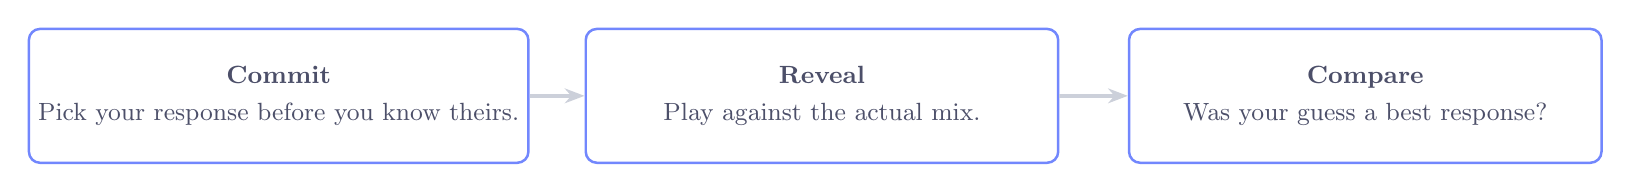
\begin{tikzpicture}[font=\small]
      \stepbox{s0}{0.0}{\textbf{Commit}\\[0.25em]
        Pick your response before you know theirs.}
      \stepbox{s1}{6.9}{\textbf{Reveal}\\[0.25em]
        Play against the actual mix.}
      \stepbox{s2}{13.8}{\textbf{Compare}\\[0.25em]
        Was your guess a best response?}
      \draw[-{Stealth[length=2.5mm]}, inkfaint, line width=1.2pt] (s0) -- (s1);
      \draw[-{Stealth[length=2.5mm]}, inkfaint, line width=1.2pt] (s1) -- (s2);
    \end{tikzpicture}

    \vspace{2.4em}

    {\large You are the \textbf{column} player throughout.}}

\newpage
\slidehead{The game}

\vspace{0.5cm}

\begin{center}
{\Large \(A = \begin{pmatrix} 2 & -2 \\ -1 & 1 \end{pmatrix}
 \qquad\qquad
 B = \begin{pmatrix} -2 & 2 \\ 1 & -1 \end{pmatrix}\)}
\end{center}

\vspace{1.1cm}

{\large \(A\) pays the row player and \(B\) pays you. Every cell adds to
\blank[1.5], so this is a \underline{\hspace{4cm}} game.}

\vspace{1.1cm}

{\large The row player will mix. You have to choose \(c_1\) or \(c_2\) before
you know how.}

\vspace{0.9cm}

\begin{center}
\workspace{22.6}{2.4}
\end{center}

\newpage
\slidehead{What you committed to}

\vspace{0.6cm}

\hspace{0.3cm}
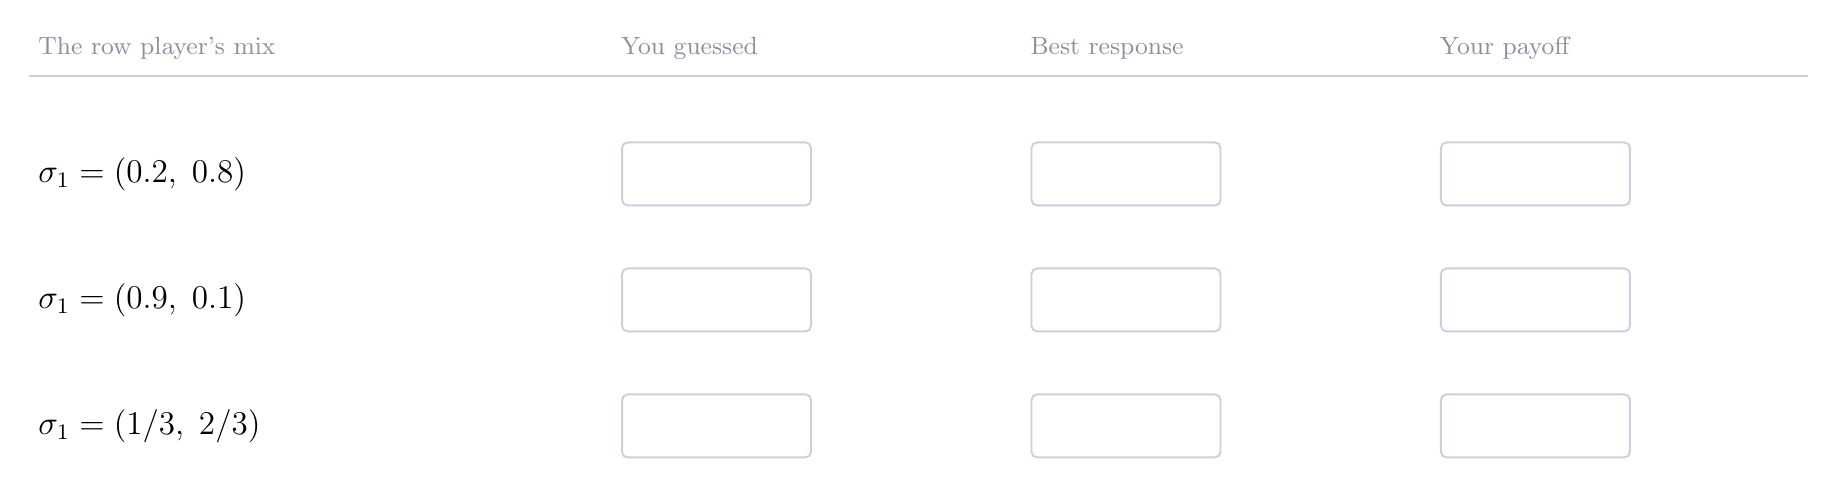
\begin{tikzpicture}[font=\small]
  \foreach \lab/\col in {The row player's mix/0, You guessed/7.4,
                         Best response/12.6, Your payoff/17.8}{%
    \node[anchor=west, text=inkgrey] at (\col,0) {\lab};}
  \draw[inkfaint, line width=0.7pt] (0,-0.36) -- (22.6,-0.36);
  \foreach \mix [count=\row from 1] in
    {{\(\sigma_1 = (0.2,\; 0.8)\)}, {\(\sigma_1 = (0.9,\; 0.1)\)},
     {\(\sigma_1 = (1/3,\; 2/3)\)}}{%
    \node[anchor=west, font=\large] at (0,-1.6*\row) {\mix};
    \node[anchor=west] at (7.4,-1.6*\row) {\blank[2.4]};
    \node[anchor=west] at (12.6,-1.6*\row) {\blank[2.4]};
    \node[anchor=west] at (17.8,-1.6*\row) {\blank[2.4]};}
\end{tikzpicture}

\vspace{0.9cm}

{\large How many pairs guessed right before the reveal? \blank[2.4]}

\newpage
\slidehead{Working it out properly}

\vspace{0.5cm}

{\large Against \(\sigma_1 = (p,\; 1 - p)\) your two actions pay}

\vspace{0.7cm}

\begin{center}
{\Large \(u_2(c_1, \sigma_1) \;=\;\) \blank[4.4] \hspace{2.2cm}
 \(u_2(c_2, \sigma_1) \;=\;\) \blank[4.4]}
\end{center}

\vspace{1.1cm}

{\large So \(c_1\) is the better reply exactly when \(p\) \blank[1.2]
\blank[1.6], and the two are equal at \(p =\) \blank[1.6].}

\vspace{0.9cm}

\begin{center}
\workspace{22.6}{2.8}
\end{center}

\newpage
\slidehead{Why dominance was no help}

\vspace{0.9cm}

{\large Is \(c_1\) dominated by \(c_2\)? \blank[2] \hspace{2.2cm}
Is \(c_2\) dominated by \(c_1\)? \blank[2]}

\vspace{1.2cm}

{\large Neither, because which one is better depends on
\underline{\hspace{6cm}}.}

\vspace{1.2cm}

{\large Dominance only settles an action that is worse against
\emph{every} strategy of the opponent. Here each action is a best response to
some mixes, so we need the \underline{\hspace{5cm}} instead.}

\vspace{1cm}

\begin{center}
\workspace{22.6}{2.4}
\end{center}

\newpage
\slidehead{The mix that makes you indifferent}

\vspace{0.8cm}

{\large At \(\sigma_1 = (1/3,\; 2/3)\) both of your actions pay \blank[1.6],
so every strategy of yours is a best response.}

\vspace{1.1cm}

{\large That is the row player's half of the equilibrium: they mix precisely so
that you cannot exploit them. Which of your own mixes does the same to
\emph{them}?}

\vspace{0.9cm}

\begin{center}
\workspace{22.6}{4.2}
\end{center}

\newpage
\slidehead{The same thing, as an exam answer}

\vspace{0.9cm}

{\large Dominance and best responses are not examined on their own. They are
examined together with \textbf{Nash Equilibrium}, so the natural follow-up is
\textbf{Question 1} on that page, where the best response condition does exactly
this job for Rock-Paper-Scissors.}

\vspace{1.4cm}

{\large The habit worth building now: before computing anything, ask which
actions could ever be a best response. Anything that never can be is not worth
carrying into the algebra.}

\vspace{1.6cm}

\begin{center}
{\large\color{inkgrey} vknight.org/gt/topics/nash-equilibrium.html}
\end{center}

\end{document}
